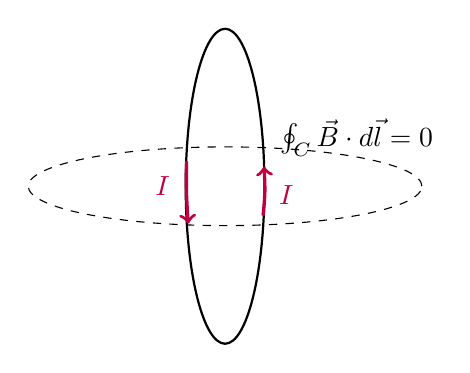
\begin{tikzpicture}

\draw  [dashed](-0.5,0.5) node (v1) {} ellipse (2.5 and 0.5);
\draw  [thick](v1) ellipse (0.5 and 2);
\draw  [very thick, ->, purple]plot[smooth, tension=.7] coordinates {(-0.0175,0.1279) (0.0052,0.4332) (-0.0061,0.7497)};
\draw  [very thick, ->, purple]plot[smooth, tension=.7] coordinates {(-0.9898,0.8176) (-0.9898,0.4106) (-0.9671,0.0262)};
\node [purple] at (-1.295,0.4979) {$I$};
\node [purple] at (0.2765,0.3849) {$I$};
\node at (1.1696,1.1186) {$\oint_C\vec{B}\cdot d\vec{l}=0$};
\end{tikzpicture}